\section{Web application honeypot}
End-user applications are an intrinsic part of an IoT infrastructure. These help users in monitoring and control IoT devices from remote locations.\\
These applications transmit user commands to the cloud, and subsequently, to IoT-enabled devices connected to the network.\\
Mobile apps, web apps, and desktop apps are the end-user applications found in an IoT infrastructure.\\
Web applications often get attacked causing a break into confidentiality and integrity of information using:
% \begin{enumerate}
\begin{itemize}
\item \textbf{SQL injection}: This is a type of attack granted by the fact that SQL doesn't check that whoever modifies the database has permission and a lack of input validation in the web application can cause the success of this attack. The attacker can insert structured Query Language code as parts of the final query string into a form that causes a web application to generate and send a query that works differently than the programmer intended;
\item \textbf{Cross-site scripting (XSS)}: An XSS allows a cracker to insert or execute client-side code to collect, manipulate and redirect confidential information, or even view and modify data on servers or alter the dynamic behavior of web pages using any language ( example JavaScript, VBScript, Flash);
\item \textbf{Remote file inclusion attacks(RFI)}: This attack is caused when an application builds a path given by the user via variable without checking its origin. The attacker modifies a user variable in the URI (example GET POST in PHP) perhaps adding malign executable code, the web application downloads and runs the remote file;
\item \textbf{Local file inclusion attacks(LFI)}: This attack is very similar to the previous one, in this case, the application only executes files included in the server so the attacker inside the script tricks the application by including another malignous script to execute.
% \end{enumerate}
\end{itemize}
In these cases, a honeypot can be very useful.\\
The Honeypot can individuate the IP source of the attack, the purpose of the attack (if there was the intention of destroying or modifying the database, etc), which methods are used by the attacker to capture data, and what is the most attacked part of the database.\\
The Web application Honeypot must respond to the attacker in the best possible way to better deceive him/her.
\subsection{DShield Web Honeypot}
The idea of this Honeypot starts with DSHield, a firewall log correlation system used by the SANS institute to collect logs received by volunteers worldwide and analyze them providing which IPs are more dangerous, which ports are more used for attacks, etc etc.\\
The honeypot is a low-latency one that collects logs from web apps adding them to all the logs that already are sent to DShield, this log contains the URL and header information such as IP address, host, user agent, referring from all requests (even harmless ones) and, after being checked with expressions in \textit{config.txt} file, they are saved inside the logs folder of the honeypot and then posting it to the DShield database (this is done every 30 minutes).\\
The honeypot works simply: on the inside, it contains a set of templates and a login system; when an attack takes place, the template is chosen checking inside the set if a suitable one is present (if there is no template, it returns a default web page), the honeypot sends the response to the attacker meanwhile the request is logged and sent to the DShield database.

\begin{figure}[h!]
\centering
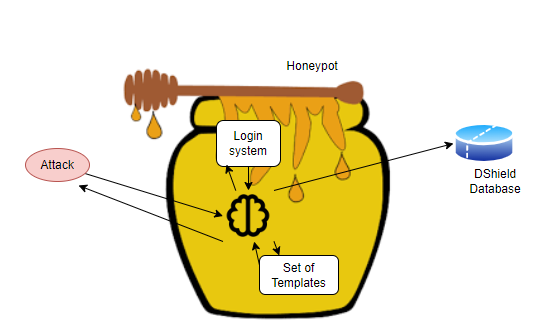
\includegraphics[width=10cm]{images/DSHoneypot.png}
\caption{Structure of DShield honeypot}
\label{fig:irradiances}
\end{figure}
\FloatBarrier


All of these ideas can be downloaded for free because all the logs are useful to the project. It is also used by home connections to collect data (as a peer-to-peer net "the more the better").

\subsection{Glastopf}
Glastopf is a very old Python web application low-interaction honeypot able to produce web applications vulnerable also to SQL injection. Glastopf manages to emulate vulnerability types, this allows us to manage multiple attacks of the same type until the attacker finds another fail in the web application or a new attack method.\\
Attackers will find the web service and try to attack the system, it is detected and gets logged by the honeypot that inserts all the information in the logs file (or database).\\
It has a good capability of logging based on the interaction that an attacker would have with the application but it shows some limitations: the front-end part is quite primary and attackers can easily recognize that this is not a real system and it only supports SQL injection, remote (RFI), and local file inclusion(LFI) vulnerabilities.

\subsection{Comparation between glastopf and DShield Honeypot}
In the paper of 2014 ,\textit{The Behavioural Study of Low Interaction Honeypots: DSHIELD and GLASTOPF in various Web Attacks}\cite{dshieldandGlastopf}, the interaction of these two honeypots with various attacks is put in comparison.\\
DShield and Galastpof have similar working techniques.
\begin{figure}[h!]
\centering
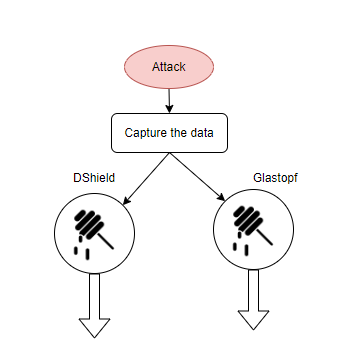
\includegraphics{images/workingtecniques.png}
\caption{Flow of attack in DShield and Galastopf}
\label{fig:irradiances}
\end{figure}
\FloatBarrier
DShield has a better ability to categorize the type of attack and utilizing the Apache server it is possible to extract a report. On the other hand, it is not easy to go through the logs and understand attacks easily.\\
Galastopf has logs that are easy to understand and they also capture the HTML information that is posted within the request, the response from the server and the response code (\texttt{200 OK}) confirming that the attack was successful on the other way cannot categorize the SQL injection and XSS and the logs generated for Remote File Inclusion attacks were lesser compared to Dshield.\\

\subsection{SNARE and Tanner}
SNARE (Super Next-generation Advanced Reactive honEypot) is a web application honeypot sensor attracting all sorts of maliciousness from the Internet.\\
It pays attention to the website, it has an inbuilt Cloner that, invoked before SNARE, clones all the web pages are given as input, all the images on the web pages, scripts and action elements so that the clone looks as good as a real system.\\
SNARE needs TANNER to work. It is a remote data analysis and classification service to evaluate HTTP requests and compose the response then served by SNARE. TANNER uses multiple application vulnerability type emulation techniques when providing responses for SNARE, so it creates each time a new session for a new attack, each session tries to detect the attacker (if it is a tool, a user, or a crawler), the location of the attack and shows through the TANNER UI for the administrator statistics regarding how many attacks of that kind have been found; after that, it emulates the response (via an emulator) and gives the attacker the response as the website would do.

\begin{figure}[h!]
\centering
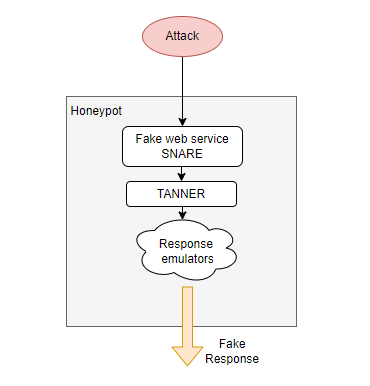
\includegraphics{images/DHP.png}
\caption{Structure of SNARE and TANNER}
\label{fig:irradiances}
\end{figure}
\FloatBarrier
\subsection{Solution of Honeypot with SNARE}

In the paper \textit{An Innovative Security Strategy using Reactive Web Application Honeypot}\cite{https://doi.org/10.48550/arxiv.2105.04773}, a solution for a web application honeypot which includes many emulators for very complex vulnerabilities is proposed. Its structure is the following manner:
\begin{enumerate}
\item SNARE: It serves all the web pages on top of itself, becoming a server and hence monitoring all the HTTP events/flows throughout the application, similar to a real system;
\item TANNER: It analyzes the requests made through SNARE after that it generates the responses dynamically;
\item Database: for attack classifications;
\item Docker: Docker is used to create containers for the emulators;
The emulator creates a container for different custom images, executes the payload of the attacker, takes the credible result, and deletes the container so that libraries are used inside a container and cannot damage the system, the honeypot remains secure;
\item Emulation engine: every event on SNARE has to pass through all types of emulators: GET, POST, and cookies emulators;
\item PHP Sandbox (PHPOX): it returns emulation results for emulators like PHP object/code injection, XXE injection, and RFI;
\item Base Emulator: it manages all the other emulators supporting multiple vulnerabilities and prepares the custom page for the injection;
\item Template Injection Emulator: this emulator imitates the Template Injection vulnerability. The input payload is matched with the element in the database to identify the type of attack, then it is injected into the docker vulnerable custom template of that type and, after the execution, the final results are sent to SNARE;
\item XML External Entity (XXE) Injection Emulator: the same story of the Template injection Emulator. It emulates XML External Entity Injection vulnerability and Out of Band XXE Injection as well;
\item PHP Object/Code Injection Emulator: it emulates the PHP Object Injection vulnerability. The injection results are sent to SNARE from the PHP sandbox so the code is executed in  the PHP sandbox safely;
\item Attacker/Crawler Detection: it allows to detect if the attacker is a crawler or a tool and tries to get the owner.
\end{enumerate}
\begin{figure}[h!]
\centering
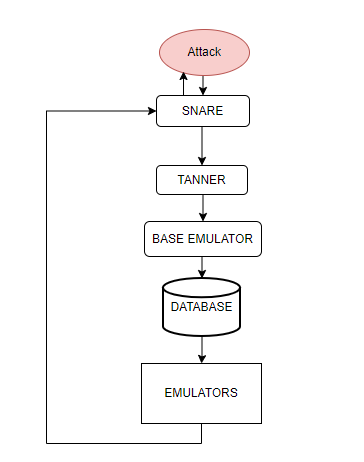
\includegraphics{images/solution.png}
\caption{Structure of the honeypot}
\label{fig:irradiances}
\end{figure}
\FloatBarrier
